\documentclass[a4paper, 12pt]{article}
\usepackage[top=2cm, bottom=2cm, left=2.5cm, right=2.5cm]{geometry}
\usepackage[utf8]{inputenc}
\usepackage[brazilian]{babel}
\usepackage{indentfirst}
\usepackage{graphicx}
\usepackage{wrapfig}
\usepackage[pdftex]{hyperref}
\graphicspath{ {imagens/} }
\usepackage{amsmath}

\begin{document}
%
\begin{titlepage} %iniciando a "capa"
	\begin{center} %centralizar o texto abaixo
		{\large Unicamp}\\[0.4cm] %0,2cm é a distância entre o texto dessa linha e o texto da próxima
		{\large Marco Lucio Bittencourt - Turma B}\\
		{\large Heitor Nigro Lopes - PED}\\[3.2cm]
		{\bf \huge Dinâmica Trabalho 2}\\[0.2cm] 
		{\bf \large Matrizes de Rotação e Range Kutta}\\[4.9cm]
		% o comando \bf deixa o texto entre chaves em negrito. O comando \huge deixa o texto enorme
	\end{center} %término do comando centralizar
	{\large Erik Yuji Goto}\\ % o comando \large deixa o texto grande
	RA: 234009\\[10cm]
	\begin{center}
	
		{\large Campinas}\\[0.2cm]
		{\large 2021}
	\end{center}
\end{titlepage} %término da "capa"


\tableofcontents
\newpage

\section{Fundição}
	\subsection{O que é fundição?}
	O processo de fundição consiste em produzir uma peça a partir do metal fundido, em estado líquido. O material é derramado em um molde e após solidificado fica com a geometria interna do molde.
	
	\subsection{Por que o processo de fundição é mais vantajoso quando comparado com outros processos de fabricação?}
	O processo de fundição tem algumas vantagens em relação aos outros processos:
	\begin{itemize}
		\item Complexidade de formas;
		\item Ampla gama de materiais;
		\item Ampla gama de propriedades;
		\item Usado para pequenos ou elevadas quantidades de peças;
		\item Baixo custo;
		\item Elevada precisão dimensional e acabamento;
		\item \textit{Near net shape} em uma única operação. 
	\end{itemize}

	\subsection{Por que a fluidez de uma liga metálica é uma propriedade importante para o processo de fundição?}
	A fluidez da liga metálica é importante, pois o material deve se depositar em todos os espaços disponível do molde. Uma liga muito visgosa pode dificultar o preenchimento interno do molde, e como resultado teremos grandes imperfeições na peça final.
	
	\subsection{Entre o ferro fundido e o aço, qual material é mais apropriado para o processo de fundição? Por quê?}
	
	\subsection{Como se chamam os dutos que conduzem o metal líquido para o interior do molde?}
	Os dutos que conduzem o metal líquido para o interior do molde se chamam canais de alimentação.
	
	\subsection{Qual o nome do reservatório que serve para suprir a peça com metal à medida que este se resfria e contrai?}
	O nome do reservatório que serve para suprir a peça com metal é \textbf{Massalote}, tem como função evitar que o interior da peça fique com 'vazios' após a solidificação da liga metálica.
	
	\subsection{Ao lado são apresentados os desenhos de uma peça fundida (fundição convencional) e da mesma peça já acabada.}
	\subsubsection{Justifique por que a peça fundida teve que ser modificada e qual a finalidade de cada modificação feita.}
	Na peça modificada não há cantos vivos, isso foi feito para facilitar a retirada da peça final do molde usado durante a solidificação. Além disso, não há furos na peça modificada, os furos foram feitos posteriormente, isso evita o uso de machos durante a fundição.
	\subsubsection{Durante a usinagem observou-se a presença de vazios. Como são chamados estes defeitos? Qual a sua causa?}
	Esses vazios são chamados porosidades. Eles ocorrem devido aos gases formados durante o processo de fundição, outra causa é a falta de massalotes. Quando há a falta de massalotes, ou quando são mal posicionados, os vazios não são alimentados com mais metal durante o resfriamento.
	\subsubsection{A ferramenta de corte esta desgastando muito rapidamente. Qual o defeito de fundição que estaria causando esse problema?}
	Como a ferramenta de corte esta desgastando muito rapidamente deve haver uma concentração de carbono na superfície da peça. Como consequência a mesma fica dura e frágil. Para reverter isso será necessário realizar um tratamento térmico.
	
	\subsection{Quais as principais diferenças entre os processos de fundição em moldes colapsáveis e processos de fundição em moldes permanentes?}
	Em processos de fundição em moldes colapsáveis o molde só é usado uma vez, pois ele é desmontado para a retirada da peça pronta, além disso o material do molde pode ser reutilizado para a produção de mais peças.
	Já os moldes permanentes podem ser usados mais de uma vez, sem a necessidade de destruir o molde e é restrito a peças de pequenas dimensões.
	
	\subsection{Qual a resistência que um molde de areia necessita ter?}
	Um molde de areia precisa ser resistente o suficiente para manter sua geometria antes e durante o processo de injeção de metal líquido.
	
	\subsection{Por que tanto o molde quanto o modelo são destruídos no processo de fundição de precisão?}
	O processo de fundição de precisão usa cera como modelo, e é envolto de cerâmica para formar o molde após endurecido. Para retirar o molde é necessário derreter a cera, destruindo assim o modelo. Depois que a liga metálica é solidificada e a peça final está quase pronta o molde de cerâmica é então colapsado. Portantom tanto o molde quanto o modelo são destruídos no processo de fundição de precisão.
	
	\subsection{Como os modelos e os moldes são produzidos no processo de fundição
de precisão?}
	\begin{itemize}
	\item Modelo: A cera é fundida em um molde metálico, depois são montados os cachos com várias peças em cera e os canais de vazamento.
	\item Molde: O molde é criado a partir do mergulho do cacho em uma suspensão cerâmica depois é colocado em um leito fluidizado de refratário. E a última etapa é a secagem do molde. Quando o molde está totalmente seco o modelo de cera é derretido, sobrando apenas o molde.
	\end{itemize}
	
	\subsection{Qual o outro nome dado ao processo de fundição de precisão?}
	O processo de fundição de precisão também é chamado de fundição por cera perdida.
	
	\subsection{Qual o princípio da fundição sob pressão?}
	Na fundição sob pressão, a liga metálica é pressionada sob baixa pressão e baixa velocidade para o interior da cavidade do molde permanente.
		
	\subsection{Quais tipos de máquinas são usados na fundição sob pressão?}
	
	\subsection{Cite duas vantagens e duas desvantagens do processo de fundição sob pressão.}
	Vantagens:	
	\begin{itemize}
		\item Não solidifica canais, portanto dispensa operações de corte
		\item Fundido livre de poros e óxidos
	\end{itemize}
	Desvantagens:
	\begin{itemize}
		\item Pressões baixas podem causar mal acabamento e outros defeitos de preenchimento
	\end{itemize}
	
	\subsection{Por que se diz que o processo “Shell Molding” (Moldagem em casa) adapta-se bem à automação?}
	
	\subsection{Qual a importância do processo de injeção de plástico no processo de fundição de precisão?}
	


\newpage
\section{Soldagem}
	\subsection{O que se entende por soldagem?}
	Soldagem é um processo de junção de peças, em que a interface das peças a serem sodladas entra em fusão. Esse tipo de processo se caracteriza por manter as propriedades químicas, físicas e metalúrgicas.
	
	\subsection{Cite duas vantagens da soldagem}
	A soldagem mantém as propriedades química, física e metalúrgica do material na região de junção. Além de ser um processo facilmente aplicável para produção em larga escala.
	
	\subsection{Em relação à tensão de soldagem nos processos de soldagem a arco, quais os significados
de: tensão em vazio, tensão de curto-circuito, tensão de soldagem}
	\begin{itemize}
		\item Tensão em vazio: Tensão da ponta da solda quando o mesmo está longe do material a ser soldado. É a tensão quando o arco elétrico está fechado.
		\item Tensão de curto-circuito: É a tensão quando o instrumento de solda se aproxima demais da peça, fazendo com que a tensão do arco elétrico diminua drásticamente e a corrente aumente muito.
		\item Tensão de soldagem: Tensão quando o arco elétrico está aberto, ou seja, quando há a existência do arco elétrico e o processo de fusão do metal acontece.
	\end{itemize}
	
	\subsection{Quais são as vantagens do processo de soldagem com eletrodo revestido?}
	\begin{itemize}
		\item É um processo versátil, podendo ser usado em vários materiais, e em qualquer posição.
		\item Custo relativamente baixo.
		\item Pode ser feito dentro de fábricas ou em campo aberto.
	\end{itemize}
	
	\subsection{Como ocorre a abertura do arco no processo de soldagem com eletrodo revestido?}
	O soldador precisa 'riscar' a peça para diminuir a tensão entre a ferramenta de solda e a peça, o que cria o arco elétrico.
	
	\subsection{Quais as vantagens da corrente alternada e da corrente contínua no processo de soldagem
com eletrodo revestido?}
	\begin{itemize}
		\item Corrente alternada(CA): tem menor queda de tensão ao longo do cabo, além disso apresenta menor desvio do arco elétrico.
		\item Corrente contínua(CC): Tem mais estabilidade do arco elétrico e maior qualidade do depósito do material de adição. Por causa disso, a maioria dos processos de soldagem com eletrodo revestido é feito em CC.
	
	\subsection{Como a corrente de soldagem influência a taxa de deposição, a largura e a profundidade
do cordão de solda, no processo de soldagem com eletrodo revestido?}
		\begin{itemize}
			\item Configuração CC-(corrente contínua com polaridade direta CCPD): Eletrodo no polo negativo e a peça no polo positivo garante maior taxa de fusão do eletrodo.
			\item Configuração CC+(corrente contínua com polaridade inversa CCPI): Eletrodo no polo positivo e a peça no polo negativo induz maior penetraçao do cordão de solda.
		\end{itemize}
		
	\subsection{De que é composto o revestimento do eletrodo?}
		\begin{figure}[h]
			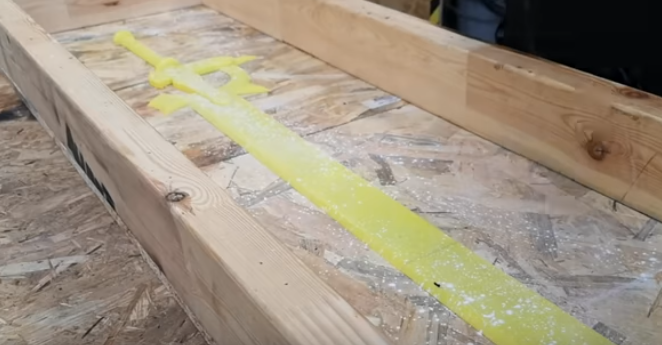
\includegraphics[scale=.5]{a.png}
		\end{figure}
		
	\subsection{Quais são as funções do revestimento do eletrodo? Dentre as várias funções, qual seria a
mais importante?}
		\begin{itemize}
			\item Estabilizar o arco elétrico.
			\item Proteger contra a ação da atmosfera
			\item Reduzir a velocidade de resfriamento do cordão de solda 
			\item Introduzir elementos de liga no cordão de solda
			
		\end{itemize}
		
		
		
		
		
		
		
		
		
		
		
		
		
		
		
		
		
		
		
		
		
		
			
	\end{itemize}		
	
	
	
	
	
	
	
	
	
	
	\begin{equation}
		Pot_{Compressor} = \frac{\dot{m}(H_2-H_1)*1000}{\eta_{compressor}}
	\end{equation}
	
\end{document}

